\section{Kerberos delegation}
\label{windows:authentication:kerberos:delegation}
{\bf Kerberos delegation allows a service to access another service on behalf
of the user}

\subsection{Delegation principle}

A web server allows a user to access his personal folder, hosted on a file
server. We are in the following situation :
\begin{figure}[!ht]
  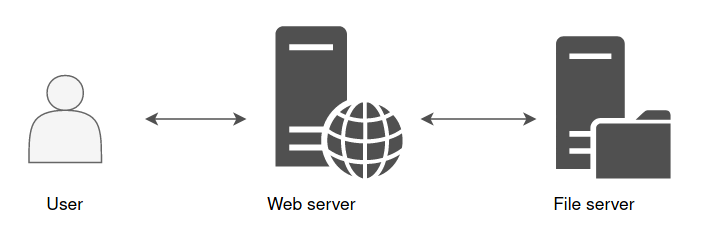
\includegraphics[width=\linewidth]{ad/knowledge/images/webfsuser.png}
  \caption{web fs user}
  \label{fig:webfsuser}
\end{figure}
The web server is front-end, and it’s this web server that will fetch the
information instead of the user on the file server in order to display the
content of a file, for example.

However, the web server does not know what belongs to the user on the file
server. It is not his role to unpack the user’s PAC to make a specific demand
to the file server. This is where the delegation comes in.

This mechanism allows the web server to {\bf impersonate} the user, and to
authenticate on the user’s behalf to the file serve.

from the file server’s point of view, it is the user who makes the request. The
file server will be able to read and check user’s rightsr, then send back the
information to which this account has access.

\begin{figure}[!ht]
  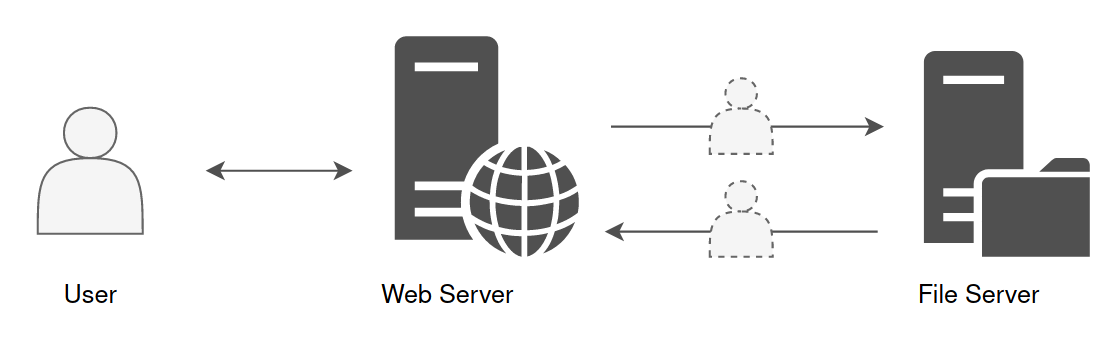
\includegraphics[width=\linewidth]{ad/knowledge/images/impersonation.png}
  \caption{Impersonation}
  \label{fig:impersonation}
\end{figure}


\subsection{Constrained \& Unconstrained Delegation}
The ability to relay credentials can be given to an {\bf account with at least
one SPN attribute set}. It could be a computer account or a service account.

there are three ways to authorize a computer or service account to impersonate
a user in order to communicate with one or more other service(s).

\subsubsection{Unconstrained Delegation}
With Unconstrained Delegation, the server or the service account that is
granted this right is able to impersonate a user to authenticate to {\bf any
services on any host}.



\begin{figure}[!ht]
  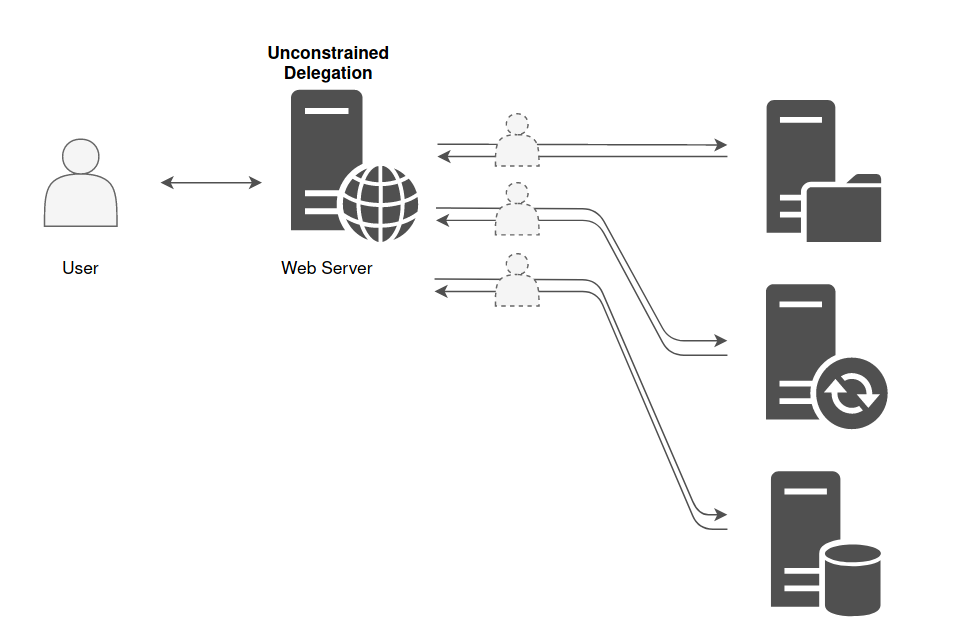
\includegraphics[width=\linewidth]{ad/knowledge/images/unconstrained_delegation_schema.png}
  \caption{Unconstrained delegation}
  \label{fig:unconstrained_delegation_schema}
\end{figure}

\subsubsection{Constrained Delegation}
If a computer or a service account has the Constrained Delegation flag set, a
list of authorized services shall be associated to this flag. 

\begin{figure}[!ht]
  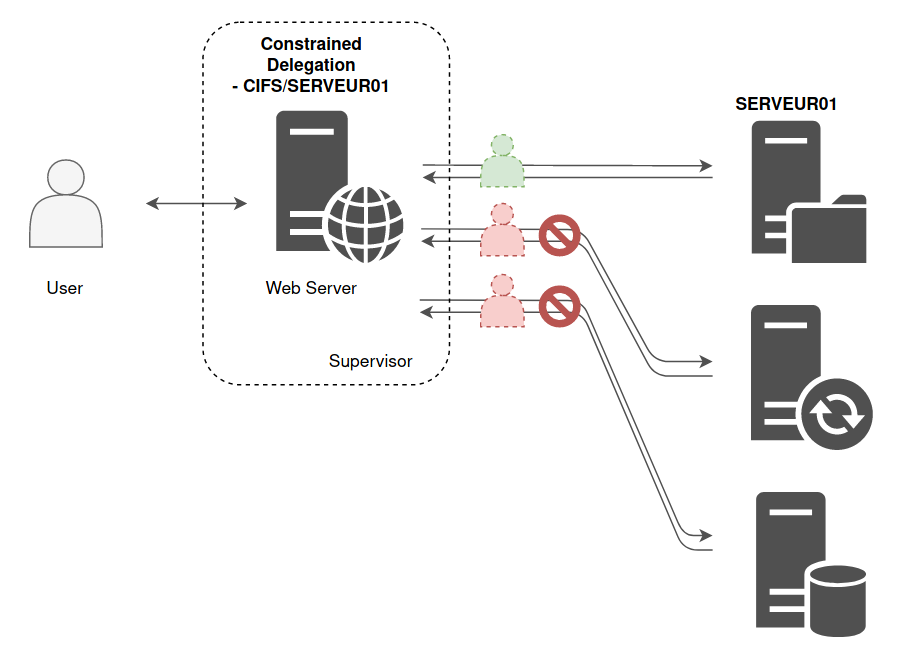
\includegraphics[width=\linewidth]{ad/knowledge/images/constrained_delegation_schema.png}
  \caption{Constrained delegation}
  \label{fig:constrained_delegation_schema}
\end{figure}

\subsection{Resource Based Delegation}
In resource based Kerberos delegation, computers (resources) specify who they
trust and who can delegate authentications to them.

This is similar to the basic constrained delegation but instead of giving
permissions to an object to impersonate any user against a service.
Resource-based Constrain Delegation sets in the object who is able to
impersonate any user against it.

Thus, the diagram is as follows :
\begin{figure}[!ht]
  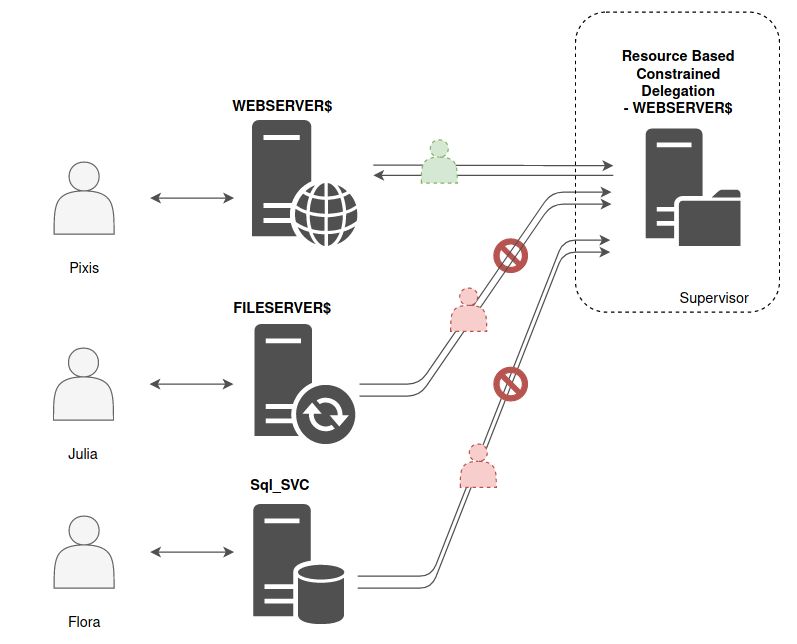
\includegraphics[width=\linewidth]{ad/knowledge/images/resource_based_constrained_delegation_schema.png}
  \caption{iRessource Based delegation}
  \label{fig:resource_based_constrained_delegation_schema}
\end{figure}
The responsibility is shifted, it’s at the level of the resource that receives
the delegated authentications that the information of whether or not the
delegation is accepted is found.

In other words, it’s the end resource that says “I allow this list of accounts
 to authenticate to me on behalf of someone else”.

In this case, the constrained object will have an attribute called
\verb+msDS-AllowedToActOnBehalfOfOtherIdentity+ with the name of the user that
can impersonate any other user against it.

Another important difference from this Constrained Delegation to the other
delegations is that any user with write permissions over a machine account
(\verb+GenericAll/GenericWrite/WriteDacl/WriteProperty/+\ldots) can set the
\verb+msDS-AllowedToActOnBehalfOfOtherIdentity+ (In the other forms of
Delegation you needed domain admin privs).


\subsection{Technical details}

\subsubsection{Unconstrained Delegation}

The \verb+UAC+ of the account as the \verb+TRUSTED_FOR_DELEGATION+ flag set (requiere \verb+SeEnableDelegationPrivilege+ to set). The user account to relay must have the \verb+UAC+ \verb+NOT_DELEGATED+ flag unset.

If both prerequisites are met, then the Domain Controller will respond to the user with a \verb+KRB_TGS_REP+ containing standard information, but it will also contains a {\bf copy of the user’s TGT} in his response, and a new associated session key.

\begin{figure}[!ht]
  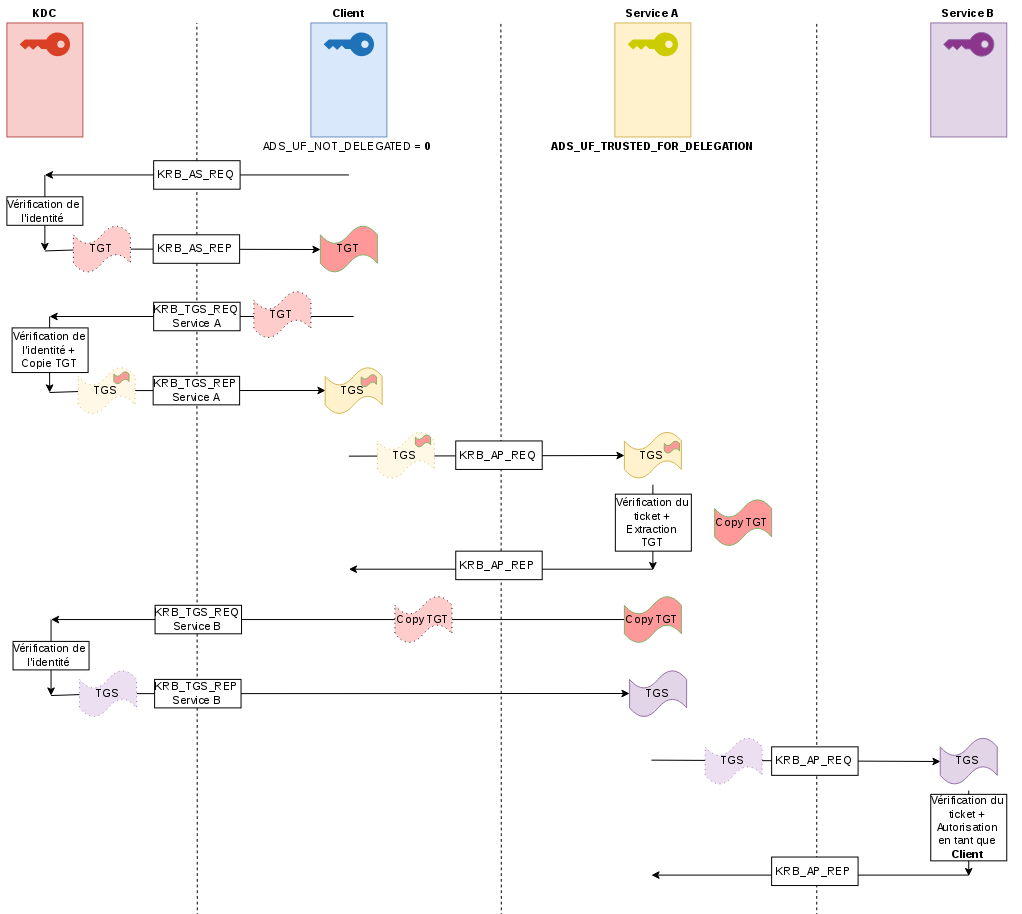
\includegraphics[width=\linewidth]{ad/knowledge/images/unconstrained_delegation_detailed.png}
  \caption{unconstrained delegation detailed }
  \label{fig:unconstrained_delegation_detailed}
\end{figure}

The service will be able to decrypt the content of the TGS, verify the user’s identity by decrypting the authenticator, but above all it will be able to retrieve the copy of the TGT and the associated session key, in order to pretend to be the user at the Domain Controller.
{\bf The TGT and the session key are stored in LSASS ?}


\subsubsection{Constrained Delegation}

\href{https://adsecurity.org/?p=1667}{Kerberos Unconstrained Delegation}
\verb+msDS-AllowedToDelegateTo+ Field of the \verb+TRUSTED_TO_AUth_FOR_DELEGATION+ account  contains the list of \verb+SPN+ the account is allow to delegate.

The user makes a TGS request, then sends it to {\emph Service A}. Since this service needs to access {\emph Resource B} as the user, it will request a \verb+TGS+ to the Domain Controller on behalf of the user. This request is governed by the \href{https://docs.microsoft.com/en-us/openspecs/windows_protocols/ms-sfu/bde93b0e-f3c9-4ddf-9f44-e1453be7af5a}{S4U2Proxy extension}. To tell the Domain Controller it wants to authenticate on behalf of someone else, two attributes will be defined in the \verb+KRB_TGS_REQ+ ticket request:
\begin{itemize}
    \item 
    The field \verb+additional-tickets+,must contain the user’s TGS (given that the \verb+NOT_DELEGATED+ flag is not set for the requesting user. If that was the case, the user’s TGS would not be forwardable, and the Domain Controller would not accept it in the rest of the process)
    \item 
    The \verb+cname-in-addl-tkt+ flag, which should be set to indicate to the Domain Controller that it should not use the server information, but the ticket information in additional-tickets.
\end{itemize}

If the targeted \verb+SPN+ is present in the \verb+msDS-AllowedToDelegateTo+, then the Domain Controller sends back a valid \verb+TGS+, with the name of the user, for the requested service.

\subsubsection{ Resource Based Delegation}

\verb+msDS-AllowedToActOnBehalfOfOtherIdentity+ of the {\emph Service B} contains the list of \verb+SPN+ allowed. The algorithm is the same except for that control.

\subsubsection{S4U2Self (transition protocol solution)}

If user authenticate to {\emph service A} without a ticket \verb+additional-tickets+ field of the \verb+TGS+ request (\verb+S4U2Proxy+) can't be set.

That is why there is an extra step, possible through the \href{https://docs.microsoft.com/en-us/openspecs/windows_protocols/ms-sfu/02636893-7a1f-4357-af9a-b672e3e3de13}{S4U2Self} extension, that {\emph Service A} must perform.

o do this, it makes a classic \verb+TGS+ request (\verb+KRB_TGS_REQ+) except that instead of putting his own name in the \verb+PA-FOR-USER+ block (present in the pre-authentication part), it puts the name of a user it chooses.

This ability to manage {\bf protocol transition} is accepted only if it has been explicitly granted to the service account wishing to manage this delegation. 

Instead of \verb+TRUSTED_FOR_DELEGATION+, \verb+TRUSTED_TO_AUTHENTICATE_FOR_DELEGATION+ must be set.

\subsection{Conclusion}

To sum up, there are three types of delegation:
\begin{itemize}
    \item 
    Unconstrained delegation: the client sends a copy of his TGT to a service, and that service uses it to impersonate the client to any other service. Only an administrator can set this option on an account.
    \item 
    Constrained delegation: A list of resources is set on the service that wishes to delegate authentication. If protocol transition is allowed, then the service can pretend to be anyone when accessing resources in its list. In any case, only an administrator can set this option.
    \item 
    Resource-based Constraint Delegation: The final resource has a list of trusted accounts. All accounts in this list can delegate authentication when accessing the resource. Resources can modify this list as they wish, they don’t need an administrator to update it.
\end{itemize}

If you have any questions or suggestions, do not hesitate, I’m all ears.

\subsection{Links}

\begin{itemize}
    \item \href{https://www.sstic.org/media/SSTIC2014/SSTIC-actes/secrets_dauthentification_pisode_ii__kerberos_cont/SSTIC2014-Article-secrets_dauthentification_pisode_ii__kerberos_contre-attaque-bordes_2.pdf}{Secrets d’authentification épisode II Kerberos contre-attaque - Aurélien Bordes}
    \item \href{https://blog.harmj0y.net/activedirectory/s4u2pwnage/}{S4U2Pwnage - Harmj0y}
    \item \href{https://shenaniganslabs.io/2019/01/28/Wagging-the-Dog.html}{Wagging the dog - Edla Shamir}
    \item 
        \url{https://book.hacktricks.xyz/windows-hardening/active-directory-methodology/constrained-delegation}
    \item 
        \url{https://www.secureauth.com/blog/kerberos-delegation-spns-and-more/}

\end{itemize}
